\documentclass[a4j,10.5pt, twocolumn]{jarticle} 
%\documentclass[a4j,10pt, twocolumn]{jarticle} 

\usepackage[dvipdfmx]{graphicx} 
\usepackage{amssymb} 
\usepackage{amsmath}
\usepackage{float}


\usepackage[compact]{titlesec}
\usepackage{fancyhdr}
\usepackage[dvipdfmx]{graphicx}
\usepackage[dvipdfmx]{color}
\usepackage{geometry}
\usepackage{pifont}
\usepackage{svg}

%---------------------------------------------------
% ページの設定
%---------------------------------------------------
%\setlength{\textwidth}{179truemm}
%\setlength{\textheight}{260truemm}
%\setlength{\topmargin}{-14.5truemm}
\setlength{\oddsidemargin}{-9.5truemm}
\pagestyle{fancy}
\fancyhf{}
\fancyhead[L]{}
\fancyhead[C]{}
\fancyhead[R]{}
\renewcommand{\headrulewidth}{0pt}
\fancyfoot[L]{}
\fancyfoot[C]{}
\fancyfoot[R]{}
\renewcommand{\footrulewidth}{0pt}
\setlength{\headheight}{12truemm}
\setlength{\parindent}{1zw}
\geometry{top=33mm,bottom=9mm,left=10mm, right=10mm}


\begin{document}
%\twocolumn
%[
%\begin{center}
 %{\huge NAISTにて取り組みたい研究について}
%\end{center}
%\vspace{5truemm}
%]

%\rhead{\parbox[b][1.8cm][b]{6cm}{\raggedleft 試験区分:情報科学区分\\氏名:夏見 昂樹\\希望研究室:自然言語処理学研究室\\現在の専門:データマイニング}}
\rhead{\parbox[b][1.35cm][b]{\textwidth}{\raggedleft 試験区分:情報科学区分\\氏名:夏見 昂樹\\希望研究室:自然言語処理学研究室\\現在の専門:データマイニング}}

\section{これまでの修学内容}
私は現在,龍谷大学先端理工学部電子情報通信課程に在学しており,データマイニング関連の研究室に所属している.3年次にはCookpadのレシピデータから手順データの利用食材と調理動作の順序性に着目することでレシピの人気分析を行った.卒業論文では-について着手する予定である.
\section{NAISTで取り組みたい研究}
\subsection{はじめに}
奈良先端科学技術大学院大学で取り組みたい研究テーマは「日本語の同音異義語誤り部にラティス構造を用いたニューラル機械翻訳の頑健性向上」である.本稿では,これまでの修学内容,研究テーマの背景・関連研究,提案手法,提案手法の評価について述べる.

\subsection{背景・関連研究}
近年,NMTモデルは目覚ましい発展を遂げているが,ほとんどのNMTモデルではノイズを含んだ入力は翻訳文に悪影響を与えてしまう\cite{Belinkov}.一般的な入力ノイズの一種として同音異義語ノイズが挙げられる.同音異義語ノイズは私たちが文章を作成時に誤った漢字変換をしてしまった際,音声入力時などに発生する.このようなノイズは入力文が膨大になるにつれ人手での検出は困難になり,翻訳時に理想的な出力を獲得するための障壁となる.

このような問題を解消するために昨今,ノイズを含んだ入力文から正確な翻訳文を獲得する研究が行われている.
Qinら\cite{Qin}は,中国語から英語の翻訳にて同音異義語ノイズのアノテーションデータが不足していることから,人工的にランダムに単語を選択し,同音異義語に置き換えることで検出器の訓練データを作成した.これを用いて同音異義語検出器を学習させ,入力文中の同音異義語誤り率の高い単語を音節に置き換えることで漢字と音節からなる混合シーケンスを作成可能とした.この混合シーケンスを扱えるように学習したNMTを用いることによって,翻訳性能とノイズに対する頑健性が向上することを示した.

本稿で取り扱う日本語に関する研究では,同音異義語の誤りを検出・訂正する手法において三品ら\cite{Mishina}は,従来のngramのみの手法に比べ,ngramと確率LSAを組み合わせることによって精度が改善することを示した.また,藤井ら\cite{Fujii}はBERTとZero-shot学習を組み合わせての検出を試みた.この他にも様々な同音異義語誤りを検出・訂正する手法が提案されているが,日本語の同音異義語誤りに頑健なNMTモデルの提案は未だ行われていない.
%\begin{figure}[ht]
   % \centering
    %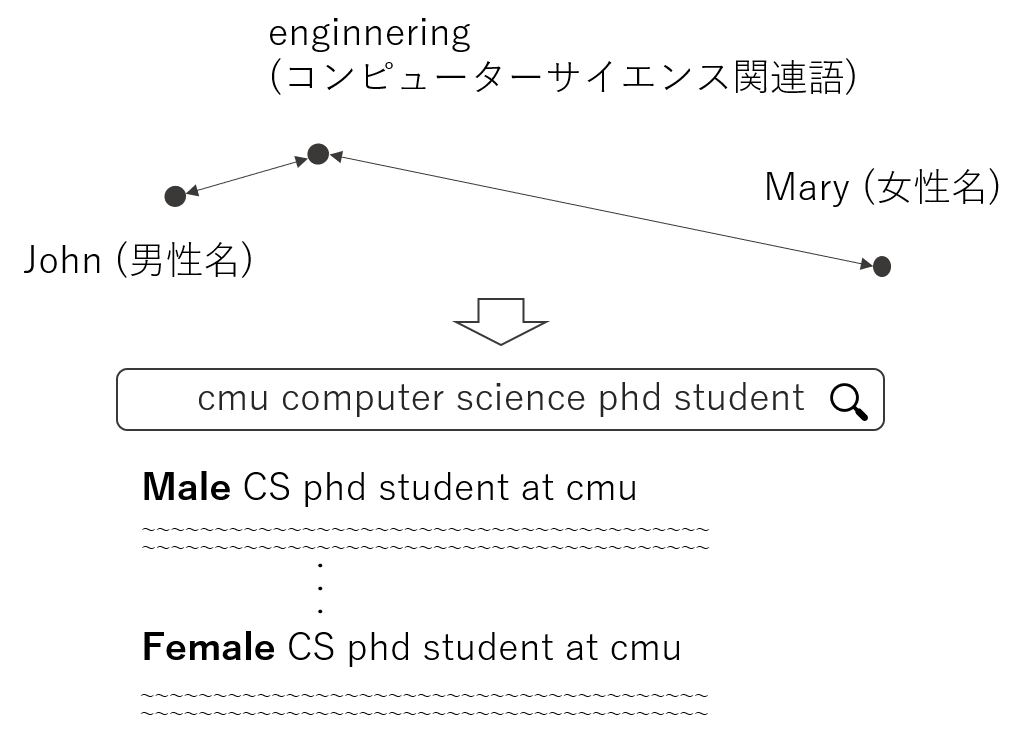
\includegraphics[width=70mm]{./bias_in_web.png}
    %\caption{バイアスのあるベクトル空間とバイアスが反映されたweb検索結果画面}
%\end{figure}

他方,NMTモデルの性能向上を図る取り組みの一例として入力シーケンスにラティス構造を取り入れる研究が行われている.しかし,近年NMTモデルとして非常に高い精度を達成したTransformerでは系列内での各トークンの位置情報を\textit{D}次元ベクトル表現に符号化する位置符号化が用いられており\cite{Vaswani},ラティス構造をそのまま入力することは困難である\cite{Xiao}.そこで,Xiaoら\cite{Xiao}はセグメンテーションの多様性がNMTの精度に影響を与えるという仮定のもと,ラティス構造を構成するノードの1文字目を絶対位置とし,ラティス構造を単一のシーケンスで表現することでTransformerへの入力を可能とした.同時にラティスグラフ同士の距離を適切に扱えるself-attentionを用いたラティスベースのエンコーダを提案し,機械翻訳タスクにて従来のTransformerエンコーダーに比べ優位性を示した.Liら\cite{Li}は中国語NERタスクにてラティス構造を構成する各トークンに始点と終点の位置を割り当てスパンからなる平坦な構造に変換することでTransformerへの入力を可能とし,従来法に比べ性能・効率ともに優れていることを示した.

このようにラティス構造をNMTに取り入れる研究は幅広く行われており,本稿で取り扱う問題の同音異義語誤りについて誤り箇所にラティス構造を用いることで,他の同音異義語候補を複数持つシーケンスを表現することが可能となる.これをNMTの入力シーケンスとして扱うことで,NMTモデルが翻訳文に基づいて複数の候補から適切な語を注視するように学習することが期待できる.

以上より私は,「BERTを用いた日本語の同音異義語誤り検出器」と「ラティス構造を含んだ入力シーケンスに対応したTransformerを用いた同音異義語に頑健な日本語から他言語へのNMTシステムの提案」を行う.

\subsection{提案手法}
提案手法は(1)同音異義語誤りの検出,(2)同音異義語誤り部へのラティス構造の付与,(3)Transformerへのラティス構造の入力・訓練,という3つのステップに分けられる.以下でそれぞれの詳細を述べる.
\subsubsection{同音異義語誤りの検出}
日本語ソース文中の同音異義語誤りを検出する手法について述べる.
検出器にはトークナイズの方法として事前学習済みモデルで文をMeCabを用いて形態素解析を行った後に単語をサブワード分割しているBERT base Japanese\footnote{https://huggingface.co/cl-tohoku/bert-base-japanese-whole-word-masking}
を用いる.また検出器の訓練データとして毎日新聞の記事データを用いる.
まず,訓練データに対して形態素解析器MeCabを用いて漢字部の読みごとの同音異義語辞書を作成する.次に先ほどMeCabによって検出された漢字部を作成した同音異義語辞書を用いて誤った同音異義語で置換することで擬似的に誤りのある文を作成する.

\begin{figure}[h]
   \centering
    \includesvg[width=88mm]{./detector.svg}
    \caption{同音異義語誤り検出手法の概略図}
\end{figure}

\begin{figure}[h]
   \centering
    \includesvg[width=88mm]{./lattice.svg}
    \caption{ラティス構造と変換後の入力シーケンス}
\end{figure}

また,我々が誤った同音異義語を選択してしまう場面は同じ同音異義語でも文中での出現頻度が低いものより高いものであるという予想から,同音異義語内を出現頻度でランキングし上位5件からランダムに選択する.加えて文中の修正箇所は3箇所までとし,この数を超えないようにランダムに選択する\footnote{これらのパラメータについては検討する必要がある}.作成された正文と誤り文を用いて各トークンごとに0(誤りなし)と1(誤りあり)の二値分類教師あり学習をBERTに対して行う.

図1は同音異義語誤りの検出手順の概略を示しており,作成した検出器からは\ding{"AC}のような出力が得らる.これをMeCabの分割に当てはめることで同音異義語誤り部を特定したいが出力はサブワードごとになるためMeCabの分割とサブワードの分割が一致するとは限らない.そこで\ding{"AD}のように一度文字レベルに0,1を割り振りを行う.最後に\ding{"AE}でMeCabの分割と検出器の出力を照らし合わせ,各分割ごとに論理和の処理を行うことで同音異義語誤り部の検出が可能となる.

\subsubsection{同音異義語誤り部へのラティス構造の付与}
検出された同音異義語誤り部に対してラティス構造を適応したシーケンスの作成手順について述べる.
まず,藤井ら\cite{Fujii}の手法に基づいて誤り部をBERTの[MASK]トークンに置き換えて,BERTに[MASK]部を予測させる処理を行う.予測結果をBERTの尤度順に10,000語取得し,それらが[MASK]部分の読みと対応する同音異義語辞書中に存在すれば,上位から最大3件抽出する\footnote{本稿では同音異義語候補を抽出する際にBERTのMLMを用いたが,純粋に同音異義語の出現頻度が高いものを数件用いるなど他の手法についても実験・評価する必要がある.}.図2(a)では上記の処理によって得られた同音異義語候補を含んだラティス構造の例を示している.この際,Qinら\cite{Qin}の入力シーケンス中に音節情報を組み込む手法を参考に,提案手法では日本語の読みをラティス構造に組み込む.これによって抽出した同音異義語候補内に正例がなかった場合であっても,NMTモデルが日本語の読みに注視して学習することを期待する.

\subsubsection{Transformerへのラティス構造の入力・訓練}
ラティス構造をNMTモデルへの入力を可能とするために,図2(b)のようにラティス構造から平文に変換することでNMTモデルへの入力を可能とする.また,NMTへのサブワード入力を可能にするために,同音異義語候補内の最長サブワード分割数の候補を基準に他の候補を左詰めで位置情報を振り分ける.これは同音異義語候補ごとにサブワード分割数が一致するとは限らないためである.

JESC,JPOなどの対訳コーパスの日本語入力文に対して提案した検出器を適応しNMTモデルを訓練する.

\subsection{提案手法の評価}
学習したNMTモデルの翻訳性能をBLEUなどによって測定し,従来のTransformerとの翻訳性能を比較することで提案モデルの翻訳性能を評価する.

提案したNMTモデルが同音異義語誤りに対して効果的か評価する必要があるが,実世界での日本語同音異義語誤りのみを取り扱った対訳データは存在しない.そこで,Qinら\cite{Qin}に基づいてテストセット内に一定の確率で人工的に同音異義語ノイズを混入させ翻訳性能を評価することでNMTモデルの同音異義語誤りへの頑健性の評価を行う.

\begin{thebibliography}{7}
{\footnotesize
\setlength{\itemsep}{-1mm}
\bibitem{Belinkov} Y. Belinkov et. al., "Synthetic and natural noise both break neural machine translation," ICLR, 2018.
\bibitem{Qin} W. Qin et. al., "Modeling Homophone Noise for Robust Neural Machine Translation," CASSP, 2021.
\bibitem{Mishina} 三品 et. al., "確率的LSAを用いた日本語同音異義語誤りの検出・訂正," 情報処理学会論文誌, 2004.
\bibitem{Fujii} 藤井 et. al., "BERTを利用したZero-shot学習による同音異義語の誤り検出," 言語処理学会 第27年次大会, 2021.
\bibitem{Vaswani} A. Vaswani et. al., "Attention is all you need," NeurIPS, 2017.
\bibitem{Xiao} F. Xiao et. al., "Lattice-Based Transformer Encoder for Neural Machine Translation," ACL, 2019.
\vspace{-0.5mm}
\bibitem{Li} X. Li et. al., "FLAT: Chinese NER Using Flat-Lattice Transformer," ACL, 2020.

\end{thebibliography}
\end{document}